\section{Размерность 4: $\chi(\R^4)\le 43$}\label{sec:main}


\subsection{Симметрийное сужение поиска}\label{ssec:symred}

Поиск оптимальной формы Грама в $\R^4$ --- задача о девяти существенных
параметрах (десять коэффициентов формы минус масштаб), и прямая оптимизация
(CMA-ES с мультистартами, \S\ref{sec:algo}) при индексах $k\le44$
устойчиво останавливалась ниже порога. Выход дало не усиление оптимизатора, а
сужение самого пространства: если потребовать, чтобы решётка допускала
\emph{заданный автоморфизм конечного порядка}, размерность задачи падает в разы.

Пусть $S\in\mathrm{GL}_4(\Z)$ --- элемент конечного порядка, а
$\Lambda$ --- решётка с $S\Lambda=\Lambda$, то есть $SQS^{\mathsf T}=Q$ для
её формы Грама. Характеристический многочлен $S$ определяет структуру модуля:
\[
\begin{aligned}
\chi_S=\Phi_3^2\ \text{или}\ \Phi_6^2
  &\ \Rightarrow\ \Z[\omega]\text{-модуль ранга }2,\\
\chi_S=\Phi_4^2
  &\ \Rightarrow\ \Z[i]\text{-модуль ранга }2,\\
\chi_S=\Phi_m,\quad \varphi(m)=4
  &\ \Rightarrow\ \Z[\zeta_m]\text{-модуль ранга }1 .
\end{aligned}
\]
Пространство $S$-инвариантных форм в первых двух случаях \emph{четырёхмерно}
(три параметра с точностью до масштаба), в третьем --- двумерно (один
параметр). Плотный скан по трём параметрам вычислительно проще, чем
случайный поиск по девяти, и --- что важнее --- он не пропускает узких
максимумов.

Дальше нам понадобится только эйзенштейнов случай $\Lambda=\Z[\omega]^2$
($\omega=e^{2\pi i/3}$). Эрмитова форма
$h=\bigl(\begin{smallmatrix}a&c\\ \bar c&b\end{smallmatrix}\bigr)$ задаёт
вещественное произведение $\langle x,y\rangle=\operatorname{Re}h(x,y)$, и в
$\Z$-базисе $(e_1,\omega e_1,e_2,\omega e_2)$ её матрица Грама
рациональна по четырём параметрам $a$, $b$, $u=\operatorname{Re}c$,
$s=\tfrac{\sqrt3}{2}\operatorname{Im}c$:
\begin{equation}\label{eq:eisform}
Q(a,b,u,s)=\begin{pmatrix}
a & -\tfrac a2 & u & -\tfrac u2-s\\[2pt]
-\tfrac a2 & a & -\tfrac u2+s & u\\[2pt]
u & -\tfrac u2+s & b & -\tfrac b2\\[2pt]
-\tfrac u2-s & u & -\tfrac b2 & b
\end{pmatrix}.
\end{equation}
Существенно, что \emph{вся} инвариантная плоскость форм определена над $\Q$:
рационализация численного оптимума не выводит из семейства и не разрушает
симметрию.

Подрешётка тоже сужается. Если требовать $S\Gamma=\Gamma$, то $\Gamma$ ---
это $\Z[\omega]$-подмодуль, а значит его индекс есть норма идеала:
в диапазоне $7\le k\le43$ допустимы лишь
\[
k\in\{7,9,12,13,16,19,21,25,27,28,31,36,37,39,43\}.
\]
Для простого
$p\equiv1\pmod3$ фактор $\Lambda/\Gamma\cong\Z[\omega]/\pi$ с $N(\pi)=p$,
поэтому $\Gamma\supseteq\pi\Lambda$ и подмодули отвечают $\mathbb F_p$-прямым
в $\Lambda/\pi\Lambda\cong\mathbb F_p^2$: их ровно $2(p+1)$. При $p=43$ это
$88$ подрешёток вместо $1+43+43^2+43^3=81\,400$ эрмитовых нормальных форм ---
перебор дешевле почти в тысячу раз, и потому скан по форме можно вести
плотно. Отметим арифметическое совпадение, без которого ничего бы не вышло:
$43=N(7+\omega)=49-7+1$ --- норма эйзенштейнова простого. Плотный скан по всем
норменным индексам показывает, что внутри этого класса порог $d=1$ впервые
достигается ровно при $k=43$: предыдущая норма $39$ даёт лишь $0{,}951$
(лестница --- \S\ref{sec:open}).

Это та же \emph{арифметическая квантизация}, что и в плоскости
(\S\ref{ssec:quant}), но этажом выше. Там она ограничивала индексы, при
которых существует подрешётка нужной формы, и снималась переходом к
нерешёточным мозаикам; здесь она ограничивает индексы, при которых существует
\emph{инвариантная} подрешётка, и ценой ей служит требование симметрии самой
$\Lambda$. Разница в том, что в плоскости квантизация мешала, а тут помогла:
именно она сузила перебор настолько, что нашёлся максимум, мимо которого
неограниченный поиск прошёл.


\subsection{Конструкция}\label{ssec:constr43}

Пусть $\Lambda_\star=B^{\mathsf T}\Z^4$, где $Q=BB^{\mathsf T}$ --- форма
\eqref{eq:eisform} с параметрами
\begin{equation}\label{eq:gram43}
a=1,\qquad b=\frac{39261}{25000},\qquad u=\frac{37381}{100000},\qquad
s=\frac{3141}{12500}
\qquad(200\,000\,Q\in\mathrm{Mat}_4(\Z)),
\end{equation}
и пусть $\Gamma_\star$ --- подрешётка индекса $43$ с матрицей перехода
(эрмитова нормальная форма; строки --- коэффициенты по базису $B$)
\begin{equation}\label{eq:hnf43}
T=\begin{pmatrix}1&0&0&41\\0&1&0&14\\0&0&1&37\\0&0&0&43\end{pmatrix},
\qquad\det T=43 .
\end{equation}
Инварианты (все рациональны, так как рациональна $Q$):
\[
\begin{aligned}
\lambda_1(\Lambda_\star)^2&=1,\\
\diam^2V_0&=\frac{5374343884337}{2019775849050}
  =2{,}660861544\ldots,\\
D(\Gamma_\star)^2&=\frac{7396075258066147}{2756867811550000}
  =2{,}682781969\ldots.
\end{aligned}
\]
\[
d(\Lambda_\star,\Gamma_\star)^2
=\frac{298768283679964998359742207}{296327113258585430253847000}
=1{,}008238093\ldots,\qquad
d=1{,}004110598\ldots
\]
Ячейка $V_0$ имеет максимально возможные $30$ фасет и $f$-вектор
$(120,240,150,30)$. В отличие от чемпиона индекса~$45$, решётка
\emph{не} общего положения: $\mathrm{Aut}(\Lambda_\star)\cong\Z/6$, три пары
кратчайших векторов вместо одной, и --- что решает дело --- вся группа
автоморфизмов сохраняет $\Gamma_\star$. Поэтому минимум $D$ достигается сразу
на трёх парах $\pm v$ орбиты $\Z/3$, а не на одной.

\begin{keybox}
\begin{theorem}\label{thm:main43}
$\chi\bigl(\R^4,[1,\ell]\bigr)\le43$ при всех $1\le\ell\le1{,}00411$;
в частности, $\chi(\R^4)\le43$.
\end{theorem}
\end{keybox}
\begin{proof}
По предложению~\ref{prop:crit} достаточно
$d(\Lambda_\star,\Gamma_\star)>\ell_0$ при $\ell_0=1{,}00411$; это неравенство
доказано в~\S\ref{sec:comp} в точной арифметике, причём двумя независимыми
способами.
\end{proof}

\begin{remark}[оптимум семейства и его структура]
Точка~\eqref{eq:gram43} --- рационализация (со знаменателем $10^5$) численного
оптимума задачи $\max d$ по трёхпараметрическому эйзенштейнову семейству. Сам
оптимум устроен как \emph{равноколебание}, и притом жёсткое: в нём
\emph{четыре} $\Z/3$-орбиты векторов $\Gamma_\star$ (двенадцать пар $\pm v$)
дают одно и то же значение $D$, а диаметр ячейки реализуется сразу на $15$
парах вершин. Четыре равные величины --- это ровно три уравнения на три
параметра, поэтому точка изолирована и условие стационарности не требуется.
В окрестности оптимума комбинаторика фиксирована (те же релевантные векторы,
та же пара вершин диаметра, те же активные грани проекций), так что
$\diam^2V_0$ и все четыре $D^2$ --- явные рациональные функции $(b,u,s)$, а
оптимум --- изолированное решение системы трёх многочленов степеней $5$, $6$,
$5$. Численно
\[
b^*=1{,}570443955560252771\ldots,\quad
u^*=0{,}438187088955734979\ldots,\quad
s^*=0{,}154716060379523302\ldots
\]
(точка определена с точностью до симметрий приведённой области: замена
$\arg c\mapsto\pi/3-\arg c$ даёт ту же решётку и те же $d$, но другие $u$, $s$),
\[
d^2=1{,}00824102343938492071\ldots,\qquad
d=1{,}00411205721243329800\ldots
\]
(значения посчитаны с $80$ верными знаками; воспроизведение ---
\path{audit-data/chromatic_research/campaigns/dim4_k43_optimum.py}).
Замкнутой формы мы не приводим: PSLQ при $80$ знаках не находит для $d^2$
минимального многочлена степени $\le8$ с коэффициентами до $10^{20}$, а прямое
исключение переменных резольвентами вырождается (результант промежуточных
многочленов степеней $28$ и $23$ обращается в нуль тождественно из-за общего
множителя). Для теоремы это и не нужно --- она стоит на рациональной точке с
сертификатом, а оптимум служит верхним ориентиром.
\end{remark}

\begin{remark}[первая найденная точка]
Исторически первой была обнаружена другая эйзенштейнова решётка того же
семейства с $200\,Q\in\mathrm{Mat}_4(\Z)$, переходом
$T=\bigl(\begin{smallmatrix}1&0&0&39\\0&1&0&13\\0&0&1&19\\0&0&0&43\end{smallmatrix}\bigr)$
и $d^2=\tfrac{14984024}{14873313}$, $d=1{,}0037149\ldots$ (сертификат
$\ell_0=1{,}003714$, файл \path{audit-data/results/cert43.json}). Она даёт ту же оценку
$\chi(\R^4)\le43$ с чуть более узким интервалом; в \S\ref{ssec:symred}
именно её симметрия и подсказала всё построение.
\end{remark}


\subsection{Более широкий интервал: $45$ и $48$ цветов}\label{ssec:wide45}

Оценка $43$ рекордна по числу цветов, но её интервал узок. Для более широких
запрещённых интервалов лучшими остаются найденные ранее решётки \emph{общего
положения} --- они не эйзенштейновы и в семейство \S\ref{ssec:symred} не
попадают. Чемпион индекса~$45$: $\Lambda_{45}=B^{\mathsf T}\Z^4$ с
\begin{equation}\label{eq:gram}
Q=\begin{pmatrix}
\tfrac{91}{15}  & \tfrac{29}{16} & -\tfrac{51}{11} & -\tfrac{55}{12}\\[3pt]
\tfrac{29}{16}  & \tfrac{123}{10}& -\tfrac{19}{4}  & -\tfrac{73}{15}\\[3pt]
-\tfrac{51}{11} & -\tfrac{19}{4} & 16              & -\tfrac{7}{5}\\[3pt]
-\tfrac{55}{12} & -\tfrac{73}{15}& -\tfrac{7}{5}   & \tfrac{139}{9}
\end{pmatrix}
\qquad(7920\,Q\in\mathrm{Mat}_4(\Z)),
\end{equation}
и подрешёткой индекса~$45$ с переходом
\begin{equation}\label{eq:hnf}
T=\begin{pmatrix}1&0&0&15\\0&1&0&41\\0&0&1&37\\0&0&0&45\end{pmatrix},
\qquad\det T=45 .
\end{equation}
Здесь $\lambda_1^2=\tfrac{91}{15}$, $\diam^2V_0\approx23{,}451$,
$D^2\approx24{,}223$, $d=1{,}016339\ldots$; ячейка тоже имеет $30$ фасет и
$f$-вектор $(120,240,150,30)$, но у $\Lambda_{45}$ \emph{единственная} пара
кратчайших векторов, $2R/\lambda_1\approx1{,}966$, и она не изометрична ни
одной классической решётке ($D_4$, $A_4^*$, $\Z^4$, $A_4$).

\begin{keybox}
\begin{theorem}\label{thm:main}
$\chi\bigl(\R^4,[1,\ell]\bigr)\le45$ при всех $1\le\ell\le1{,}015$, и
$\chi\bigl(\R^4,[1,\ell]\bigr)\le48$ при всех $1\le\ell\le1{,}0396$.
\end{theorem}
\end{keybox}
\begin{proof}
Как и выше: точные сертификаты неравенств $d>\ell_0$ для обеих форм ---
файлы \path{audit-data/results/cert45.json} и
\path{audit-data/results/cert48.json}; схема
проверки описана в~\S\ref{sec:comp}.
\end{proof}

Три ступени вместе (полная таблица ширин --- \S\ref{sec:wide}):
\[
\begin{array}{lccc}
\text{цветов} & 43 & 45 & 48\\
\ell\le & 1{,}00411 & 1{,}015 & 1{,}0396\\
\text{решётка} & \text{эйзенштейнова} & \text{общего положения} & \text{общего положения}
\end{array}
\]
Ширина здесь --- расходуемый ресурс (\S\ref{sec:product}), поэтому в
произведениях блок с $45$ цветами полезнее блока с $43$: $1/1{,}015^2=0{,}971$
оставляет запас бюджета, а $1/1{,}00411^2=0{,}9918$ --- практически нет.

\begin{remark}[почему прежний поиск не находил $43$]
Рис.~\ref{fig:descent} показывает <<спуск>> по числу цветов. Кампания
2026-07 (CMA-ES по всем девяти параметрам формы, восемь независимых
запусков на $k=44$ и лишь три на $k=43$) дала максимумы $0{,}990$ при $k=44$ и
$0{,}971$ при $k=43$ и была честно записана как отрицательный экран.
Она оказалась не препятствием, а недобором статистики: эйзенштейнов максимум
$1{,}00411$ лежит в области, куда ни один из трёх стартов не попал. Урок
методический, а не арифметический: в задачах такого рода полезнее сузить
пространство поиска симметрией, чем наращивать число рестартов в полном.
Плотный скан \emph{всего} эйзенштейнова семейства (\S\ref{ssec:symred})
при $k<43$ порога не достигает --- см. \S\ref{sec:open}.
\end{remark}

\begin{figure}[t]
\centering
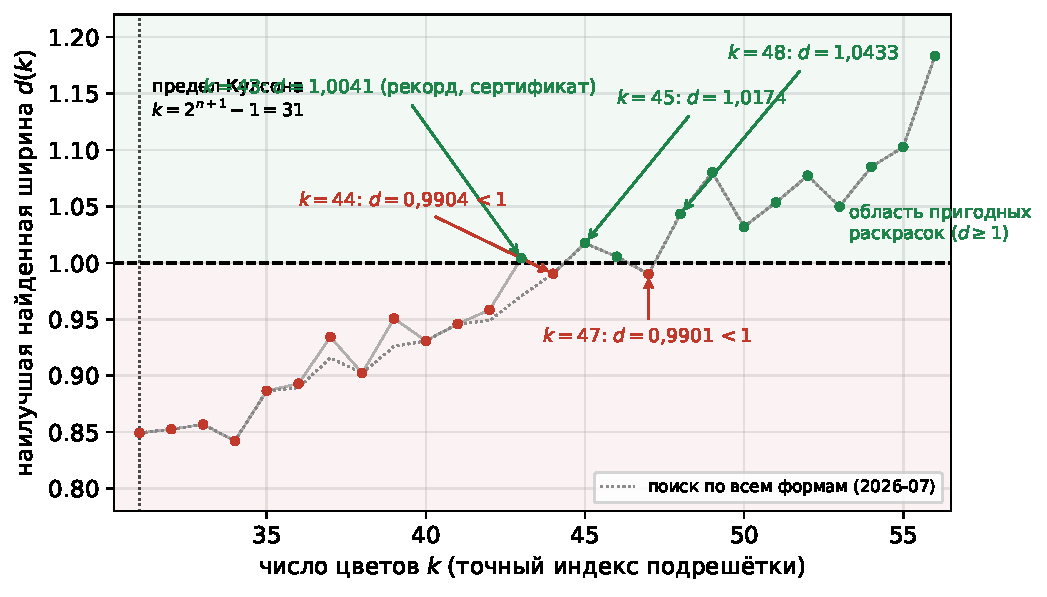
\includegraphics[width=0.74\textwidth]{fig_descent.pdf}
\caption{Наилучшая найденная нормированная ширина $d(k)$ при \emph{точном}
индексе подрешётки $k$. Зелёные точки ($d\ge1$) отвечают пригодным
раскраскам, красные --- нет. Рекорд --- индекс $43$ на эйзенштейновой решётке
($d=1{,}004111$); при $44\le k\le48$ показаны оптимумы поиска по всем формам.
Немонотонность отражает теоретико-числовую структуру: число доступных
подрешёток зависит от разложения $k$, поэтому <<богатые>> составные индексы
($45=3^2\!\cdot5$, $48=2^4\!\cdot3$) и эйзенштейновы нормы ($43=N(7+\omega)$)
пробиваются легче. Серым --- кампания 2026-07 по общим формам, остановившаяся
на $d\le0{,}990$ при $k\le44$; пунктир --- предел Кулсона $k=31$.}
\label{fig:descent}
\end{figure}


\subsection{Точный сертификат неравенства $d>\ell_0$}\label{sec:comp}

Неравенство $d>\ell_0$ проверено \emph{в точной рациональной арифметике}
двумя независимыми способами. Первый (опорный) заменяет недоступный в
замкнутой форме многогранник $V_0$ на объемлющий $P\supseteq V_0$ с
рациональными вершинами; второй считает те же величины точно и без
объемлющего многогранника. Проверкой служит согласие: диаметры совпали как
дроби, а опорная оценка снизу на $D^2$ оказалась не больше точного значения
(и обе величины перекрывают порог $\ell_0^2\diam^2$).

\paragraph{Способ 1: опорные оценки.}
Пусть $P$ --- пересечение $30$ полупространств-биссекторов
$\{x:\langle x,v\rangle_Q\le\tfrac12\langle v,v\rangle_Q\}$ по $15$ парам
целочисленных релевантных векторов $\pm v$. Каждый биссектор содержит $V_0$,
поэтому $V_0\subseteq P$, и обе нужные оценки идут в безопасную сторону:
$\diam V_0\le\diam P$ и $\dist(p,V_0)\ge\dist(p,P)$.
\begin{enumerate}[leftmargin=1.8em]
\item[(а)] \textbf{Диаметр сверху.} Все вершины $P$ перечислены точно (решение
$\binom{30}{4}=27\,405$ рациональных систем $4\times4$ с проверкой всех
неравенств; вершин ровно~$120$), откуда для формы~\eqref{eq:gram43}
$\diam^2V_0\le\diam^2P=\tfrac{5374343884337}{2019775849050}
=2{,}660861544\ldots$
\item[(б)] \textbf{Расстояние снизу.} Для каждого вектора $v\in\Gamma_\star$ в
доказуемо полном окне~\eqref{eq:window}: либо точно
$\langle v,v\rangle_Q\ge W^2$ с рациональным $W^2\ge(1+\ell_0)^2\diam^2P$
(тогда $D(v)\ge\|v\|-\diam V_0\ge\ell_0\diam V_0$ автоматически, так как
$\diam V_0=2R$ для центрально симметричной ячейки), либо --- для $12$ коротких
кандидатов --- применяется опорное неравенство
\[
\dist(v/2,P)\ \ge\
\frac{\langle v/2,u\rangle_Q-\max_{w\in\mathrm{vert}\,P}\langle w,u\rangle_Q}
{\|u\|_Q}
\]
с рациональным направлением $u$. Все величины --- точные дроби; в итоге
\[
D(\Gamma_\star)^2\ \ge\ \frac{869307639027355969}{324032161065600000}
=2{,}682781969\ldots
\]
\item[(в)] \textbf{Вывод.} $\ell_0^2\diam^2P=2{,}682778773\ldots$, и так как
$2{,}682781969>2{,}682778773$, получаем $D(\Gamma_\star)^2>\ell_0^2\diam^2V_0$,
то есть $d>\ell_0$ строго. \qed
\end{enumerate}

\paragraph{Способ 2: точный пересчёт без объемлющего многогранника.}
Здесь $V_0$ строится сам, а не заменяется на $P$: релевантные векторы
находятся по теореме Вороного (минимумы нормы в $15$ ненулевых смежных классах
$\Lambda/2\Lambda$), вершины --- тем же перебором четвёрок, а расстояние
$\dist(v/2,V_0)$ вычисляется \emph{точно}: активное множество берётся из
плавающей точки, а оптимальность подтверждается условиями Каруша--Куна--Таккера
в дробях (допустимость $x^*$ и неотрицательность множителей). Контроль
построения --- центральная симметрия множества вершин и равенство
$\vol V_0=\det\Lambda$. Результат --- не оценка, а сами величины
$\diam^2V_0$, $D^2$ и $d^2$, выписанные выше: диаметр совпал с~(а) как дробь,
а $D^2=\tfrac{7396075258066147}{2756867811550000}$ оказался, как и должно,
чуть больше опорной оценки~(б).
Плавающая арифметика в обоих способах используется лишь для \emph{выбора}
кандидатов, направлений и активных множеств --- на строгость это не влияет.

Дополнительно исчерпывающим перебором всех $81\,400$ подрешёток индекса~$43$
подтверждено, что~\eqref{eq:hnf43} доставляет максимум $d$ для
$\Lambda_\star$, а перебором всех $188\,760$ подрешёток индекса~$45$ ---
что~\eqref{eq:hnf} максимальна для $\Lambda_{45}$.
